\begin{frame}
  \frametitle{Implementing the Fault Detector}
  \begin{itemize}
    \item Build a convolutional neural network in DL4J
      \begin{itemize}
        \item Easy to monitor training and compute evaluation metrics
        \item Fast due to C++ backend engine
      \end{itemize}
    \item First, data has to be normalized
      \begin{itemize}
        \item Activation levels can vary across superlayers
        \item We only care about the distinct fault patterns
        \item Scale wire activations from 0 to 1
      \end{itemize}
    \item Many architectures and parameters were tried
      \begin{itemize}
        \item Network too shallow \(\rightarrow\) unable to learn
          complex faults (e.g. two dead wires next to each other)
        \item Multiple faults per superlayer are possible
          \(\rightarrow\) multiple networks were trained, each
          specializing in a single fault
      \end{itemize}
  \end{itemize}
\end{frame}

\begin{frame}
  \frametitle{Final Network Architecture}
  \begin{figure}
    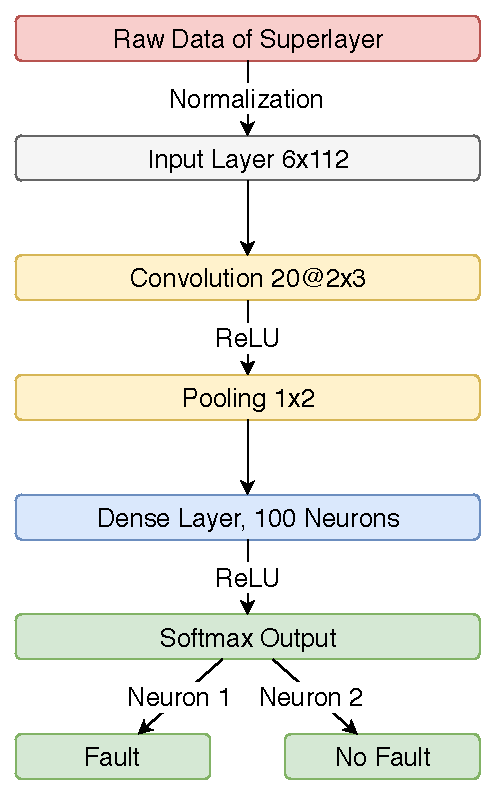
\includegraphics[height=.8\textheight]{../figures/fault_architecture}
  \end{figure}
\end{frame}

\begin{frame}
  \frametitle{Training the Fault Detector}
  \begin{itemize}
    \item Used Michaels simulation suite
      \begin{itemize}
        \item Based on real world background signals
        \item Randomly inserts fault combinations and generates labels
          accordingly
      \end{itemize}
    \item Each classifier was trained on 100,000 examples
    \item Testing was done using 10,000 new examples from the
      simulator
      \begin{itemize}
        \item Accuracy was always above 97\%
      \end{itemize}
  \end{itemize}
  \begin{figure}
    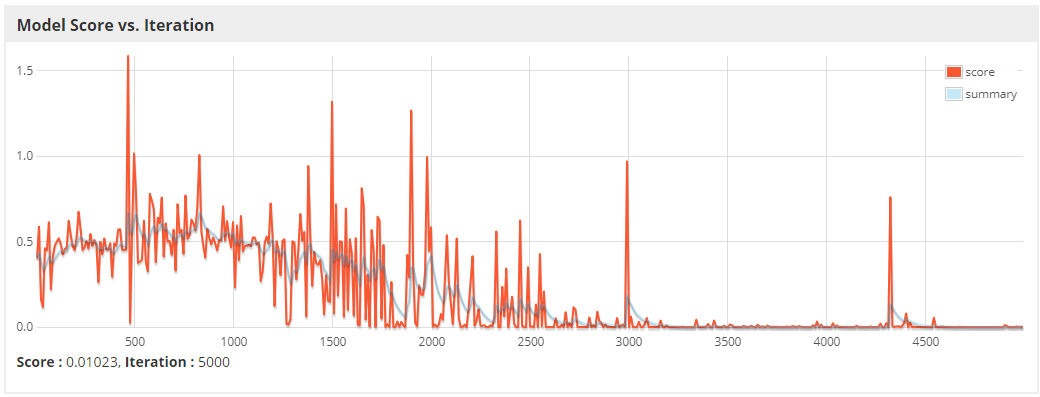
\includegraphics[width=.85\textwidth]{../figures/learning_curve}
  \end{figure}
\end{frame}

\begin{frame}
  \frametitle{Real Data Validation}
  \begin{itemize}
    \item Need to show that the detector not only works on simulated
      data
      \begin{itemize}
        \item Did it extract some general concepts?
      \end{itemize}
    \item Tested the system on some real world examples to show its
      strengths and weaknesses
  \end{itemize}
\end{frame}

\begin{frame}
  \frametitle{Pin Fault and Dead Wires}
  \begin{figure}
    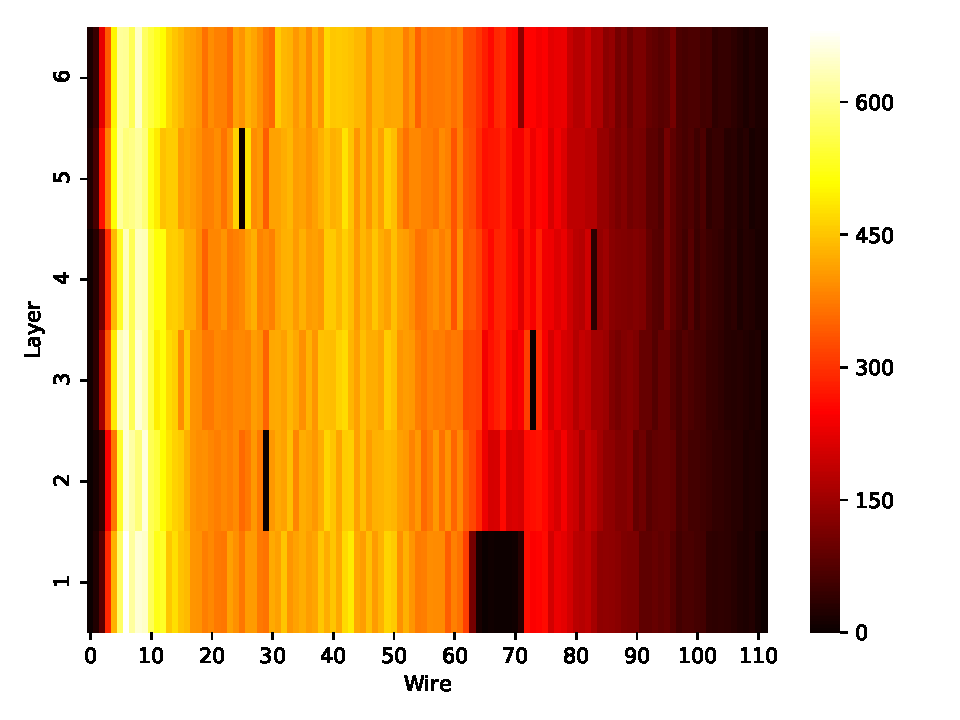
\includegraphics[width=.64\textwidth]{../figures/small_pin_success}
  \end{figure}
  \begin{itemize}
    \item Faults display a sharp contrast \(\rightarrow\) classifier
      works well
      \begin{itemize}
        \item Dead pin and dead wire classifier both report 100\%
          fault
        \item The other classifiers don't detect their
          fault with 99\% certainty
      \end{itemize}
  \end{itemize}
\end{frame}

\begin{frame}
  \frametitle{Blurred Dead Pin Fault}
  \begin{figure}
    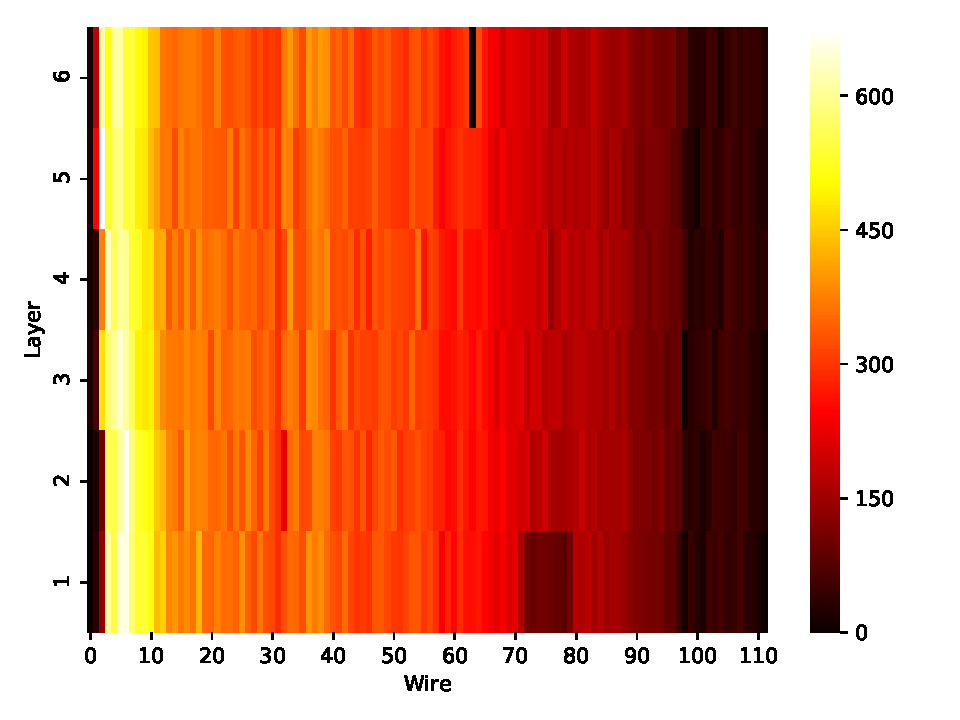
\includegraphics[width=.64\textwidth]{../figures/small_pin_fail}
  \end{figure}
  \begin{itemize}
    \item Blurred fault \(\rightarrow\) classifier struggles
      \begin{itemize}
        \item Classifier reports 99\% no fault for the pin
        \item We believe that more real data can solve this
      \end{itemize}
  \end{itemize}
\end{frame}

\begin{frame}
  \frametitle{Two Dead Wires}
  \begin{figure}
    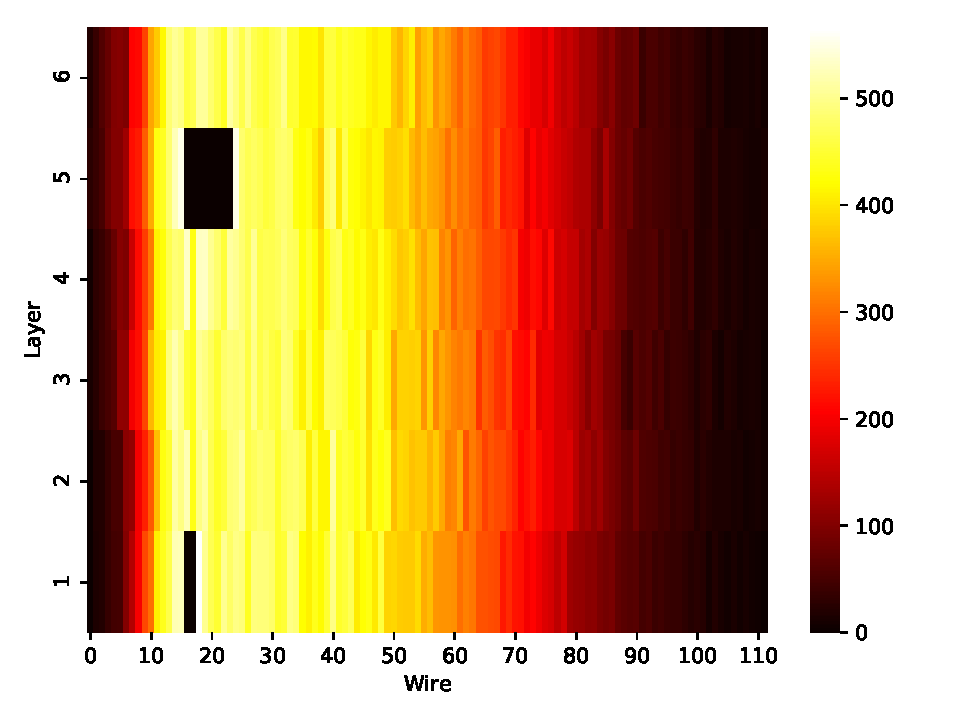
\includegraphics[width=.64\textwidth]{../figures/two_wires}
  \end{figure}
  \begin{itemize}
    \item Classifier detects two dead wires next to each other
      \begin{itemize}
        \item Reports 93.29\% certainty for the wires and 100\% for
          the pin
      \end{itemize}
  \end{itemize}
\end{frame}
